\section{High-level design description}
\subsection{Requirement specification}
\begin{itemize}
 \item Ein Simpler Rechner mit den folgenden Operationen:
	\begin{itemize}
	 \item Addition
	 \item Subtraktion
	 \item Multiplikation
	 \item Division
	\end{itemize}
 \item I/O
 	\begin{itemize}
 	 \item PS/2 Keyboard als Eingabemodul
 	 \item VGA Monitor als Ausgabemodul
 	 \item RS232 Upload der 50 zuletzt eingegebenen Berechnungen
 	\end{itemize}
 \item Arithmetische Ausdruecke\\
	Es werden folgende arithmetischen Eingaben unterstützt und nach der Konvention
		der Operatorrangfolge abgearbeitet:
 	\begin{itemize}
 	 \item Digits:     0...9
 	 \item Operatoren: +, -, *, /
 	\end{itemize}
 \item Funktionelle Ausdruecke\\
 	Des Weiteres sollen folgende Funktionalen Ausdruecke unterstuetzt werden\\
 	 Backspace, Enter, Space
 \item Fehlerbehandlung
	Folgende Eingaben werden zu Abbruch bzw. zur Fehlerausgabe führen. Daraus folgt die Abspeicherung 
		eines Error Codes.
	\begin{itemize}
 	 \item Division durch 0
	 \item Ungültige Positionierung von Operanden (Anfang, Ende, zwei in Serie)
	 \item Overflows von Zahlen und Berechnungen
	\end{itemize}

\end{itemize}



\subsection{Decomposition in submodules (schematic)}
\begin{figure}[!ht]
 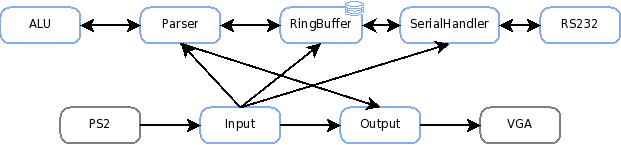
\includegraphics[scale=0.55]{pics/Modules.png}
 % Modules.png: 501x145 pixel, 72dpi, 17.67x5.12 cm, bb=0 0 501 145
 \label{fig:Modules}
\end{figure}

%\subsection{Interface definition}
\subsection{Testcase specification}
%%%%%%%%%%%%%%%%%%%%%%%%%%%%%%%%%%%%%%%%%%%%%%%%%%%%%%%%%%%%%%%%%%%%5

\begin{enumerate}
 \item TC1 : Addition zweier Zahlen
 \item TC2 : Subtraktion zweier Zahlen
 \item TC3 : Multiplikation zweier Zahlen
 \item TC4 : Division zweier Zahlen
 \item TC5 : Verkettung aller Grundrechnungsarten
 \item TC6 : Punkt vor Strichrechnung
 \item TC7 : zu große Zahlen verwenden
 \item TC8 : Division durch 0
 \item TC9 : zwei Operatoren hintereinander, 
 \item TC10 : Operator am Ende
 \item TC11 : Überlange Eingabe
 \item TC12 : Leertase erzeugt einen Abstand der bei der Berechnung ignoriert wird.
 \item TC13 : Backspace l�scht uns das letzte Zeichen
 \item TC14 : Auslesen der History
 \item TC15 : Fehlermeldung f�r Division durch Null
 \item TC16 : Fehlermeldung f�r einen Syntax Fehler
 \item TC17 : Fehlermeldung f�r einen Overflow
 \item TC18 : Divisionen werden abgerundet

\end{enumerate}


% \begin{itemize}
% \item TC1: adding two positive numbers – covers requirement 1,3,6
% \item TC2: erroneous input (too large numbers, … ) - covers requirement 2,7
% \end{itemize}
